%!TEX encoding = UTF-8 Unicode
% -*- coding: UTF-8; -*-
% vim: set fenc-utf-8

\chapter{Fils de fer}
\label{s:fil_fer}

Ce chapitre présente les maquettes des principales interfaces de l'application VisuaLigue.
Une courte explication des fonctionnalités moins évidentes est également présente à la suite des figures si nécessaire.

\begin{figure}[htpb]
    \centering
    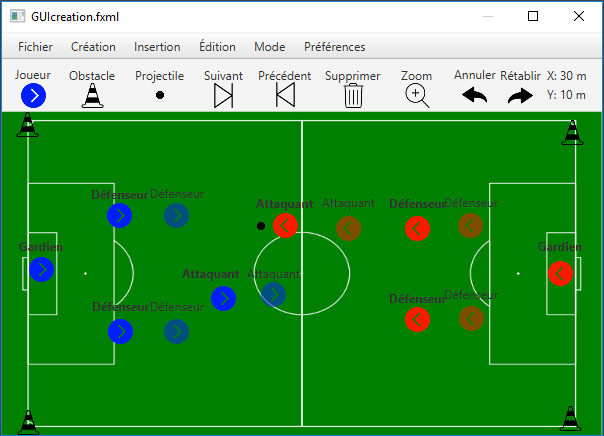
\includegraphics[scale=0.7]{fig/gui/gui_creation.png}
    \caption{Interface pour la création des stratégies}
    \label{fig:gui:gui_creation}
\end{figure}

\begin{figure}[htpb]
    \centering
    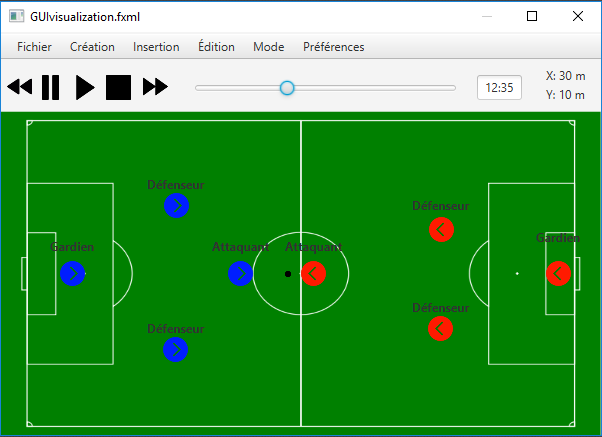
\includegraphics[scale=0.7]{fig/gui/gui_visualisation.png}
    \caption{Interface pour la visualisation des stratégies}
    \label{fig:gui:gui_visualisation}
\end{figure}

\begin{figure}[htpb]
    \centering
    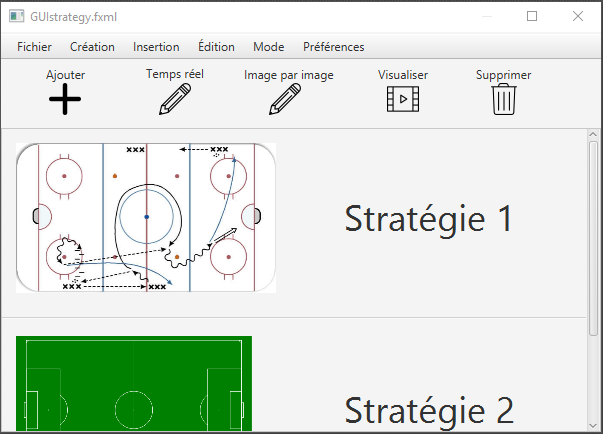
\includegraphics[scale=0.7]{fig/gui/gui_strategie.png}
    \caption{Interface de gestion des stratégies}
    \label{fig:gui:gui_strategie}
\end{figure}

\begin{figure}[htpb]
    \centering
    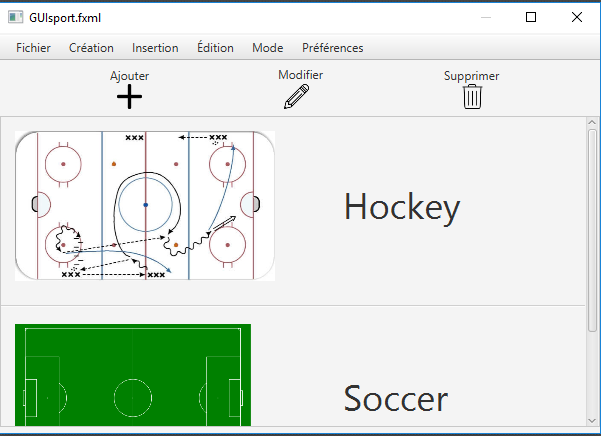
\includegraphics[scale=0.7]{fig/gui/gui_sport.png}
    \caption{Interface de gestion des sports}
    \label{fig:gui:gui_sport}
\end{figure}

\begin{figure}[htpb]
    \centering
    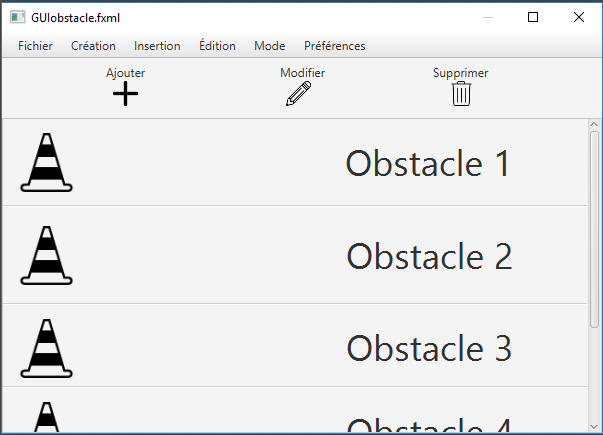
\includegraphics[scale=0.7]{fig/gui/gui_obstacles.png}
    \caption{Interface de gestion des obstacles}
    \label{fig:gui:gui_obstacles}
\end{figure}

\begin{figure}[htpb]
    \centering
    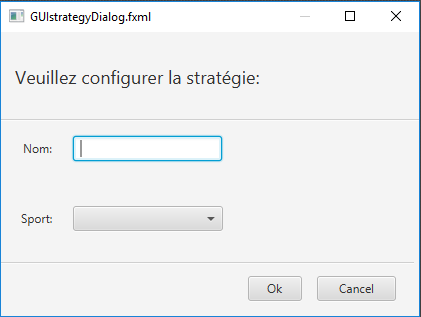
\includegraphics[scale=0.7]{fig/gui/gui_strategie_dialog.png}
    \caption{Interface de configuration des stratégies}
    \label{fig:gui:gui_strategie_dialog}
\end{figure}

\begin{figure}[htpb]
    \centering
    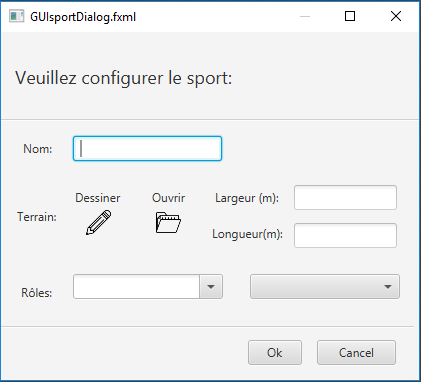
\includegraphics[scale=0.7]{fig/gui/gui_sport_dialog.png}
    \caption{Interface de configuration des sports}
    \label{fig:gui:gui_sport_dialog}
\end{figure}

\begin{figure}[htpb]
    \centering
    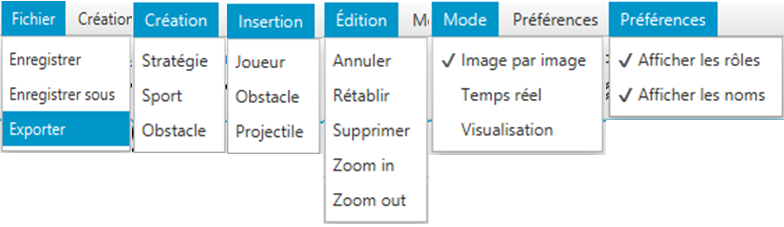
\includegraphics[scale=0.7]{fig/gui/gui_menu.png}
    \caption{Interface du menu pour montrer les options}
    \label{fig:gui:gui_menu}
\end{figure}
